\begin{figure}[ht]
 \centering
 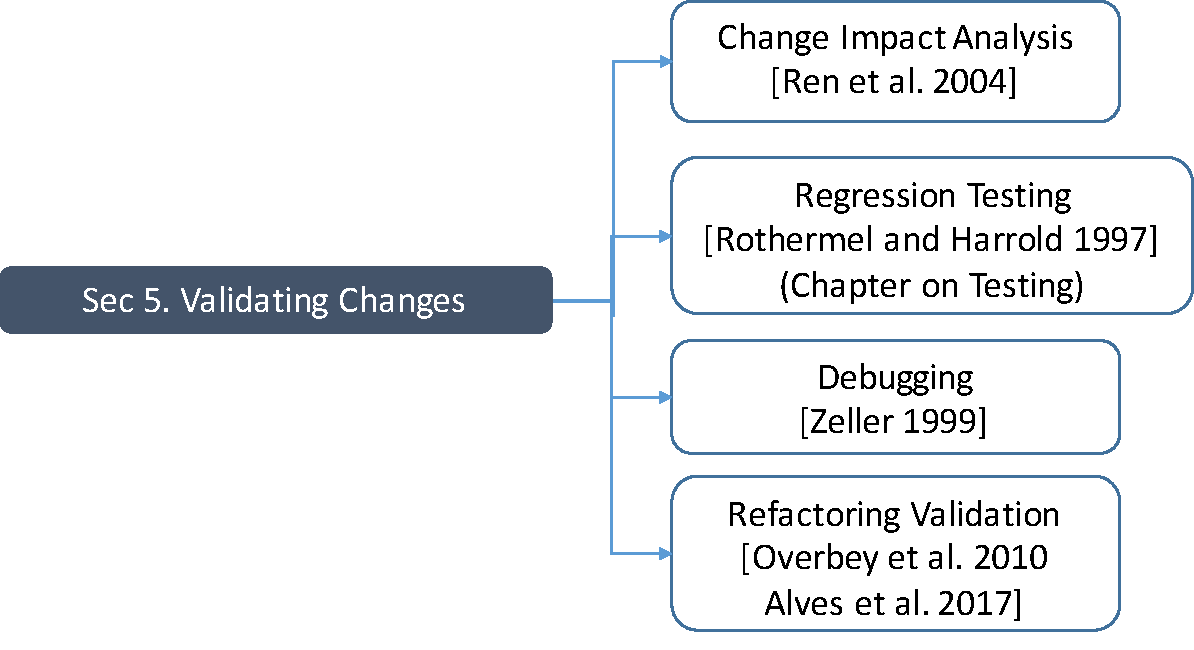
\includegraphics[width=0.6\textwidth]{images/ChangeValidation.pdf} 
 \caption{Change Validation and Related Research Topics} 
 \label{fig:changevalidation} 
\end{figure}

After making software changes, developers must validate the correctness of updated software. Validation and verification is a vast area of research. In this section, we focus on techniques that aim to identify faults introduced due to software changes. As Chapter~\todo{cross reference to testing} discusses the history and seminal work on regression testing in details, we refer the interested readers to that chapter instead. Section~\ref{sec:CIA} discusses Change Impact Analysis, which aims to determine the impact of source code edits on programs under test. Section~\ref{sec:deltadebugging} discusses how to localize program changes responsible for test failures. Section~\ref{sec:refactoringvalidation} discusses the techniques that are specifically designed to validate refactoring edits under the assumption that software's external behavior should not change after refactoring. 

\subsection{Change Impact Analysis} 
\label{sec:CIA} 
Change Impact Analysis consists of a collection of techniques for determining the effects of source code modifications, and can improve programmer productivity by: (i) allowing programmers to experiment with different edits, observe the code fragments that they affect, and use this information to determine which edit to select and/or how to augment test suites, (ii) reducing the amount of time and effort needed in running regression tests, by determining that some tests are guaranteed not to be affected by a given set of changes, and (iii) reducing the amount of time and effort spent in debugging, by determining a safe approximation of the changes responsible for a given test’s failure. 

In this section, we discuss the seminal change impact analysis work, called Chianti that serve the both purposes of affected test identification and isolation of failure-inducing deltas. 
It uses a two-phase approach in Figure~\ref{fig:twophase}~\cite{Ren2004}. 

In the first phasee, to identify which test cases a developer must rerun on the new version to ensure that all potential regression faults are identified, Chianti takes the old and new program versions $P_o$ and $P_n$ and an existing test suite $T$ as inputs, and identify a set of atomic program changes at the level of methods, fields, and subtyping relationships. It then computes the profile of the test suite $T$ on $P_o$ in terms of dynamic call graphs and selects $T'\subset T$ that guarantees the same regression fault revealing capability between $T$ and $T'$. 

In the second phase, Chianti then first runs the selected test cases $T'$ from the first phase on the new program version $P_n$ and computes the profile of $T'$ on $P_n$ in terms of dynamic call graphs. It then uses both the atomic change set information together with dynamic call graphs to identify which subset of the delta between $P_o$ and $P_n$ led to the behavior differences for each failed test on $P_n$. 

\begin{figure*}
\centering
\begin{minipage}{.45\textwidth}
  \centering
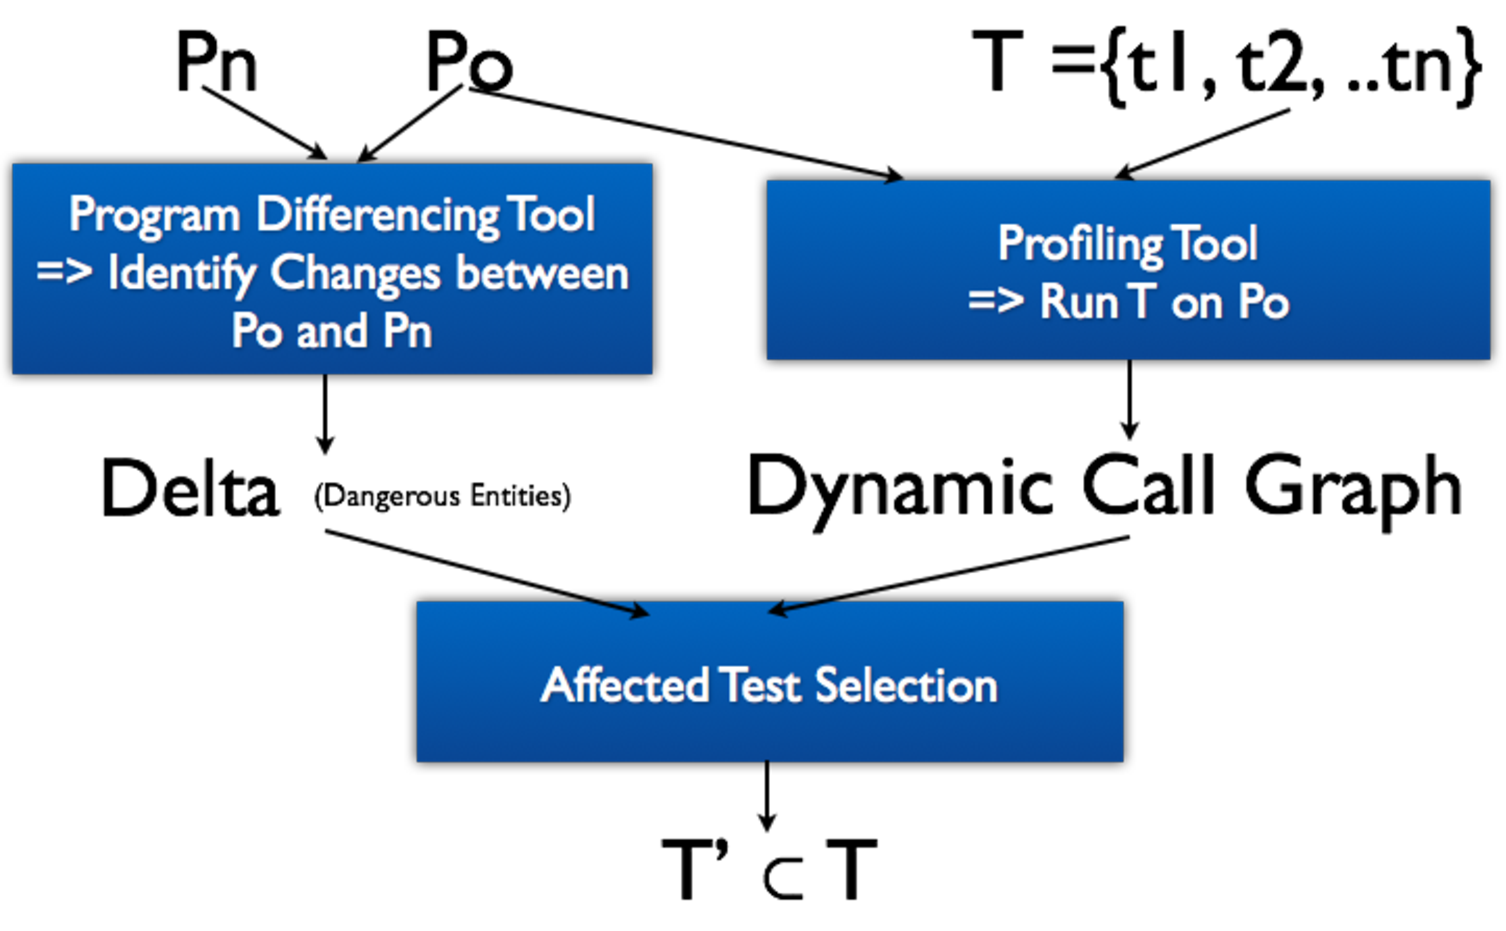
\includegraphics[width=0.9\textwidth]{images/ChiantiPhase1.pdf}
\end{minipage}
\begin{minipage}{.45\textwidth}
  \centering
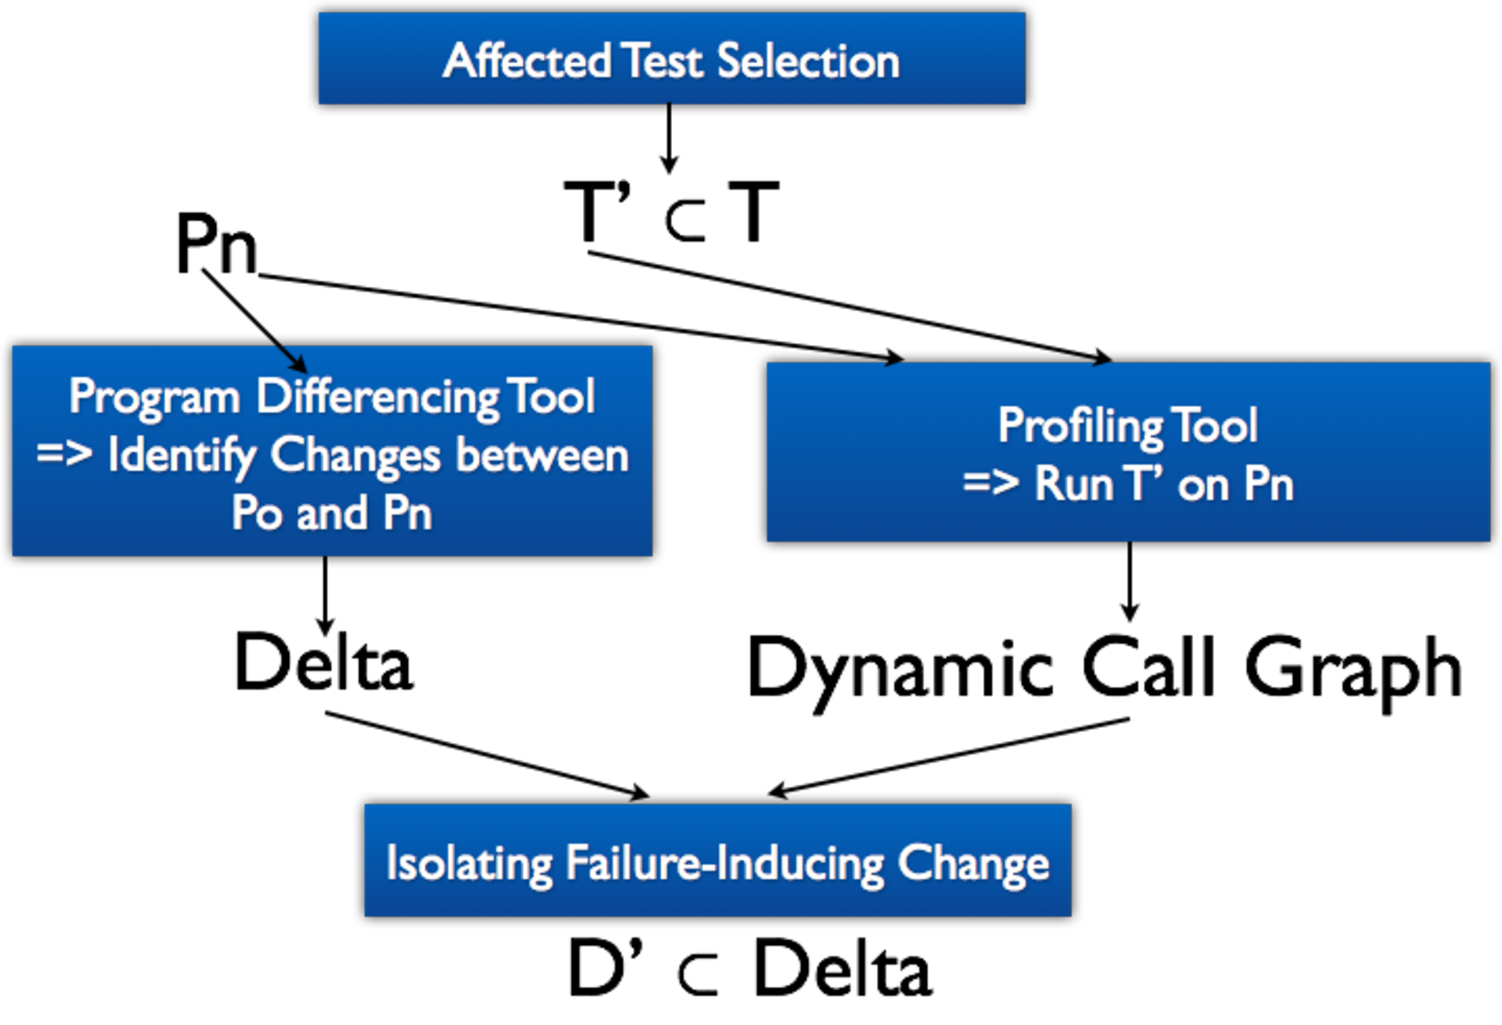
\includegraphics[width=0.9\textwidth]{images/ChiantiPhase2.pdf}
\end{minipage}:w

\caption{Chianti Change Impact Analysis: identifying affected tests (left) and identifying affecting change (right)~\cite{Ren2004}} 
\label{fig:twophase} 
\end{figure*}

To represent atomic changes, Chianti compares the syntax tree of the old and new program versions and decomposes the edits into atomic changes at a method and field level. Changes are then categorized as added classes (AC), deleted classes (DC), added methods (AM), deleted methods (DM), changed methods (CM), added fields (AF), deleted fields (DF), and lookup (i.e., dynamic dispatch) changes (LC). The LC atomic change category models changes to the dynamic dispatch behavior of instance methods. In particular, an LC change \codefont{LC(Y, X.m())} models the fact that a call to method \codefont{X.m()} on an object of type \codefont{Y} results in the selection of a different method call target.

For example, Figure~\ref{fig:chianti} shows a software change example and corresponding lists of atomic changes inferred from AST-level comparison. An arrow from an atomic change $A1$ to an atomic change $A2$ indicates that $A2$ is dependent on $A1$. For example, the addition of the call \codefont{B.bar()} in method \codefont{B.foo()} is the method body change \codefont{CM(B.foo())} represented as \textcircled{8}. This change \codefont{8} requires the declaration of method \codefont{B.bar()} to exist first, i.e., \codefont{AM(B.bar())} represented as \textcircled{6}. This dependence is represented as an arrow from \textcircled{6} to \textcircled{8}. 

Phase I reports {\bf affected tests}\textemdash a subset of regression tests relevant to edits. It identifies a test if its dynamic call graph on the old version contains a node that corresponds to a changed method (CM) or deleted method (DM)  or or if the call graph contains an edge that corresponds to a lookup change (LC). Figure~\ref{fig:chianti} also shows the dynamic call graph of each test for the old version (left) and the new version (right). Using the call graphs on the left, it is easy to see that: (i) \codefont{test1} is not affected, (ii) \codefont{test2} is affected because its call graph contains a node for \codefont{B.foo()}, which corresponds to \textcircled{8}, and (iii) \codefont{test3} is affected because its call graph contains an edge corresponding to a dispatch to method \codefont{A.foo()} on an object of type \codefont{C}, which corresponds to \textcircled{4}. 

Phase II then reports {\bf affecting changes}\textemdash a subset of changes relevant to the execution of affected tests in the new version. For example, we can compute the affecting changes for \codefont{test2} as follows. The call graph for \codefont{test2} in the edited version of the program contains methods \codefont{B.foo()} and \codefont{B.bar()}. These nodes correspond to \textcircled{8} and \textcircled{9} respectively. Atomic change \textcircled{8} requires \textcircled{6} and \textcircled{9} requires \textcircled{6} and \textcircled{7}. Therefore, the atomic changes affecting test2 are \textcircled{6}, \textcircled{7}, \textcircled{8}, and \textcircled{9}. Informally, this means that we can automatically determine that \codefont{test2} is affected by the addition of field \codefont{B.y}, the addition of method \codefont{B.bar()}, and the change to method \codefont{B.foo()}, but not on any of the other source code changes. 

\begin{figure*}
\centering
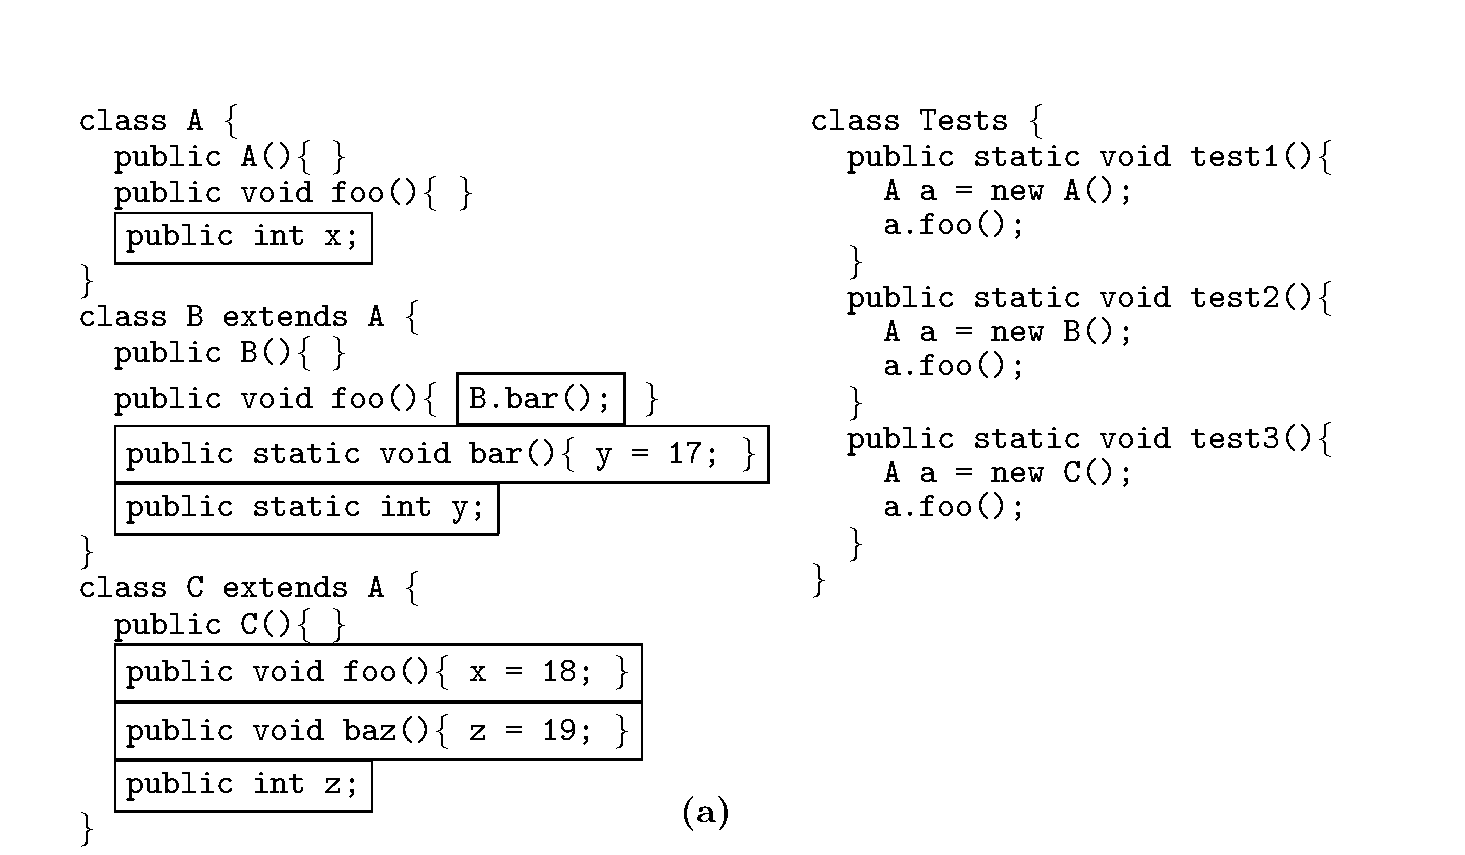
\includegraphics[width=0.95\textwidth]{images/ChiantiExample.pdf}
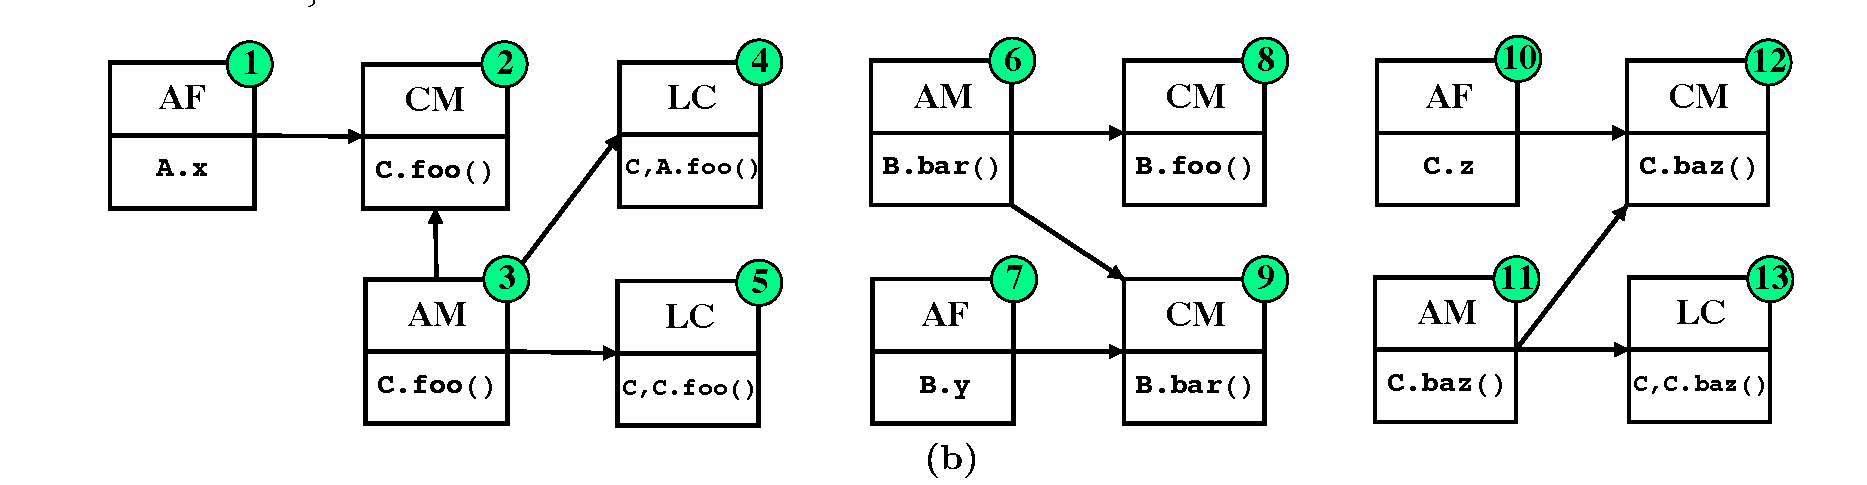
\includegraphics[width=0.95\textwidth]{images/ChiantiAtomicChange.pdf}

\includegraphics[width=0.9\textwidth]{images/DynamicCallGraph.png}
\caption{Chianti change impact analysis} 
\label{fig:chianti} 
\end{figure*}

\subsection{Debugging Changes} 
\label{sec:deltadebugging} 
The problem of simplifying and isolating failure-inducing input is a long standing problem in software engineering. {\it Delta Debugging (DD)} addresses this problem by repetitively running a program with different sub-configurations (subsets) of the input to systematically isolate failure-inducing inputs~\cite{Zeller1999, zeller01}. DD splits the original input into two halves using a binary search-like strategy and re-runs them.  DD requires a test oracle function $test(c)$ that takes an input configuration $c$ and checks whether running a program with $c$ leads to a failure.  If one of the two halves fails, DD recursively applies the same procedure for only that failure-inducing input configuration. On the other hand, if both halves pass, DD tries different sub-configurations by mixing fine-grained sub-configurations with larger sub-configurations (computed as the complement from the current configuration). 

Under the assumption that failure is {\em monotone}\textemdash where $C$ is a super set of all configurations, if a larger configuration $c$ is successful, then any of its smaller sub-configurations $c'$ does not fail, i.e., $\forall c \subset C\ (\ test(c)=\text{\cmark} \rightarrow \forall c' \subset c \  (test(c') \neq$ \ding{55})), DD returns a minimal failure-inducing configuration. Figure~\ref{fig:deltadebugging} shows the pseudo-code of DD and the illustration of isolating failure-inducing inputs. 

\begin{figure*}
\centering
\begin{minipage}{.48\textwidth}
  \centering
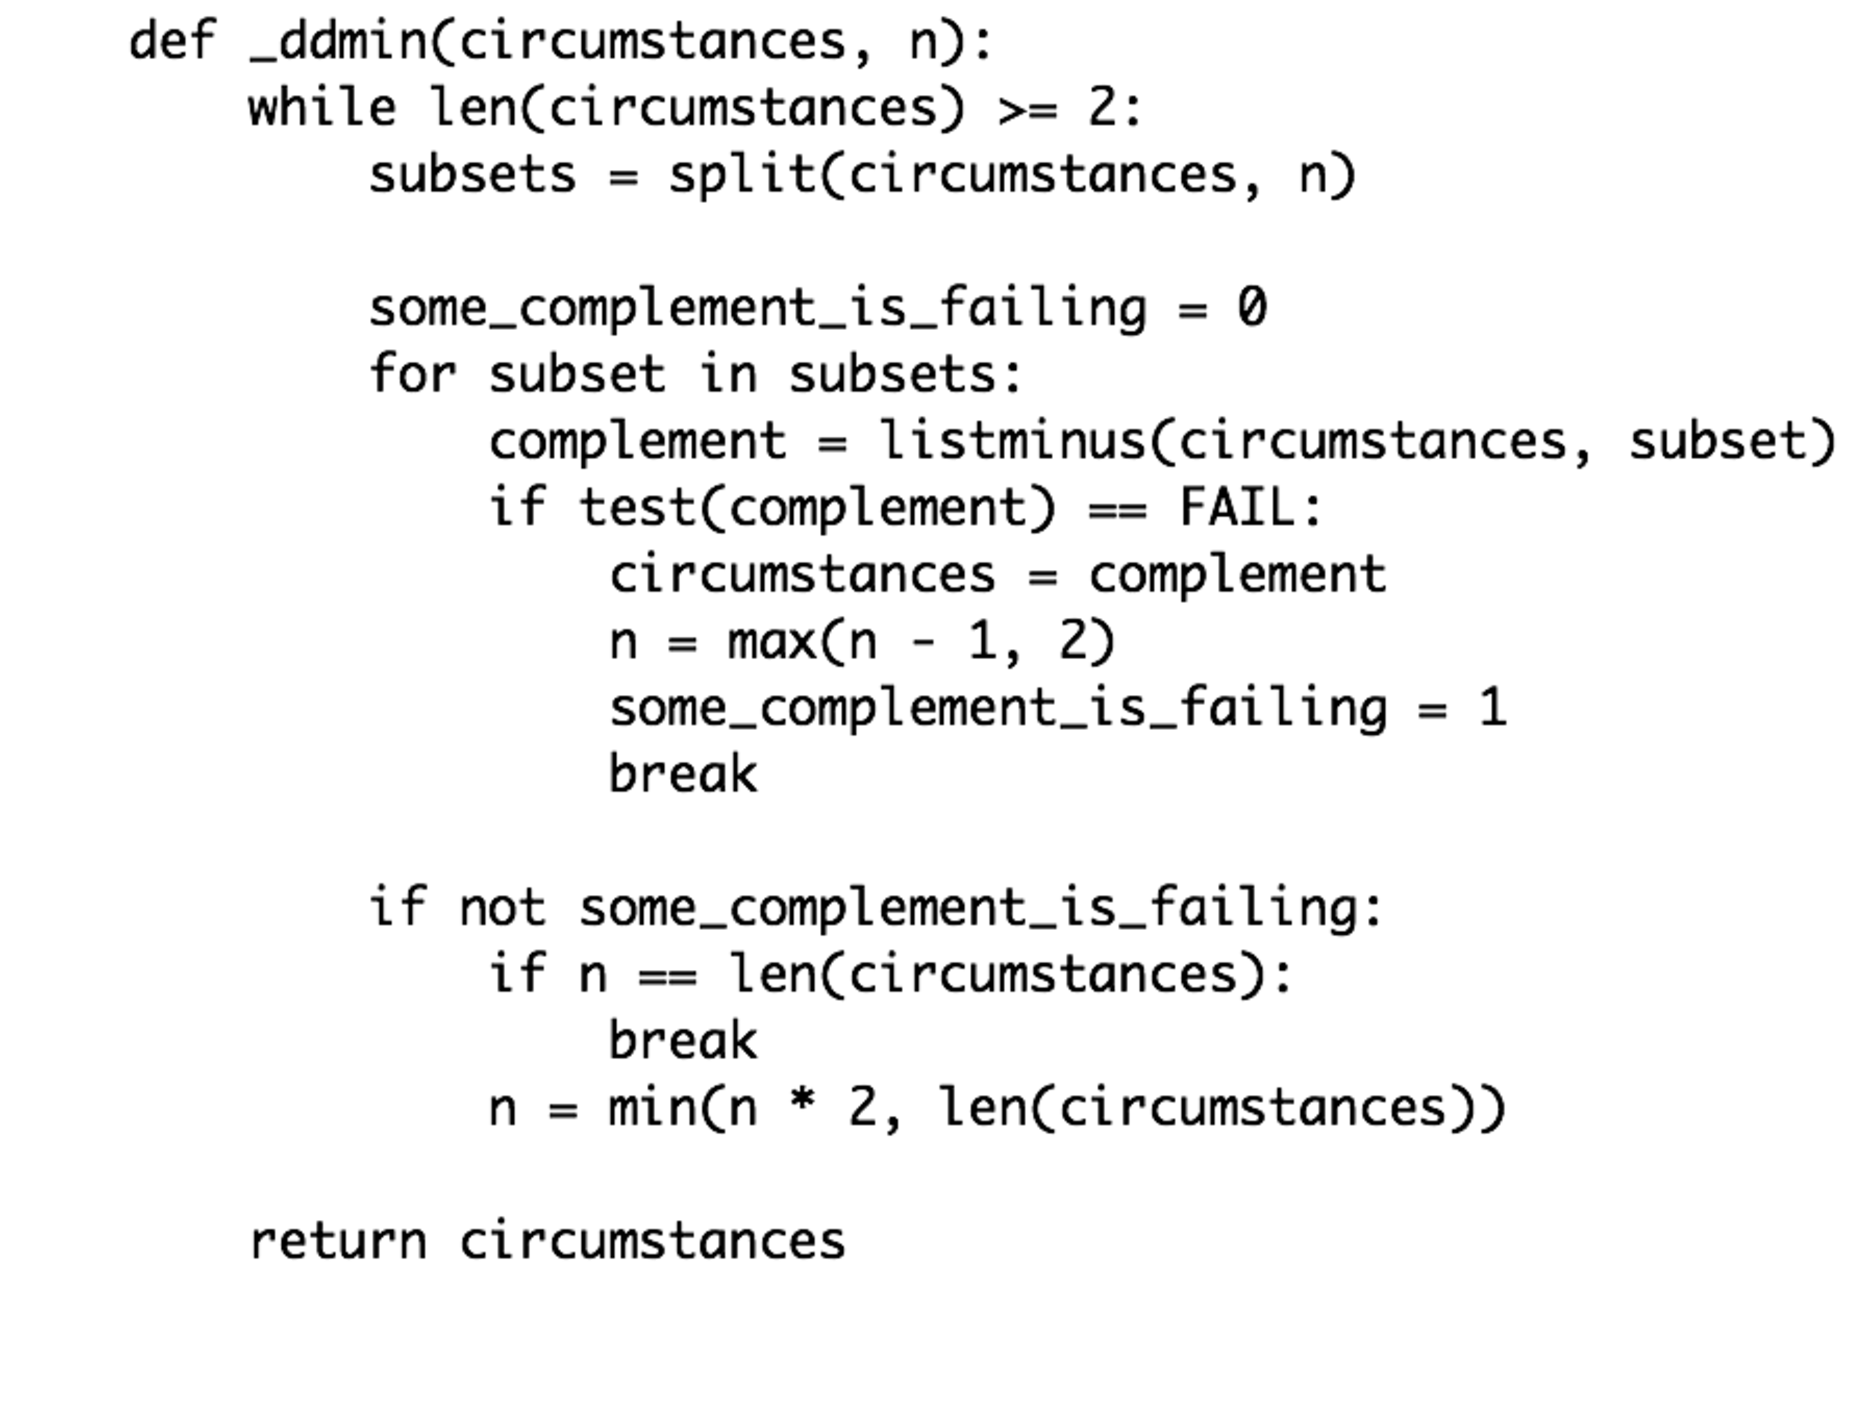
\includegraphics[width=1\textwidth]{images/DeltaDebugging.pdf}
\end{minipage}
\begin{minipage}{.48\textwidth}
  \centering
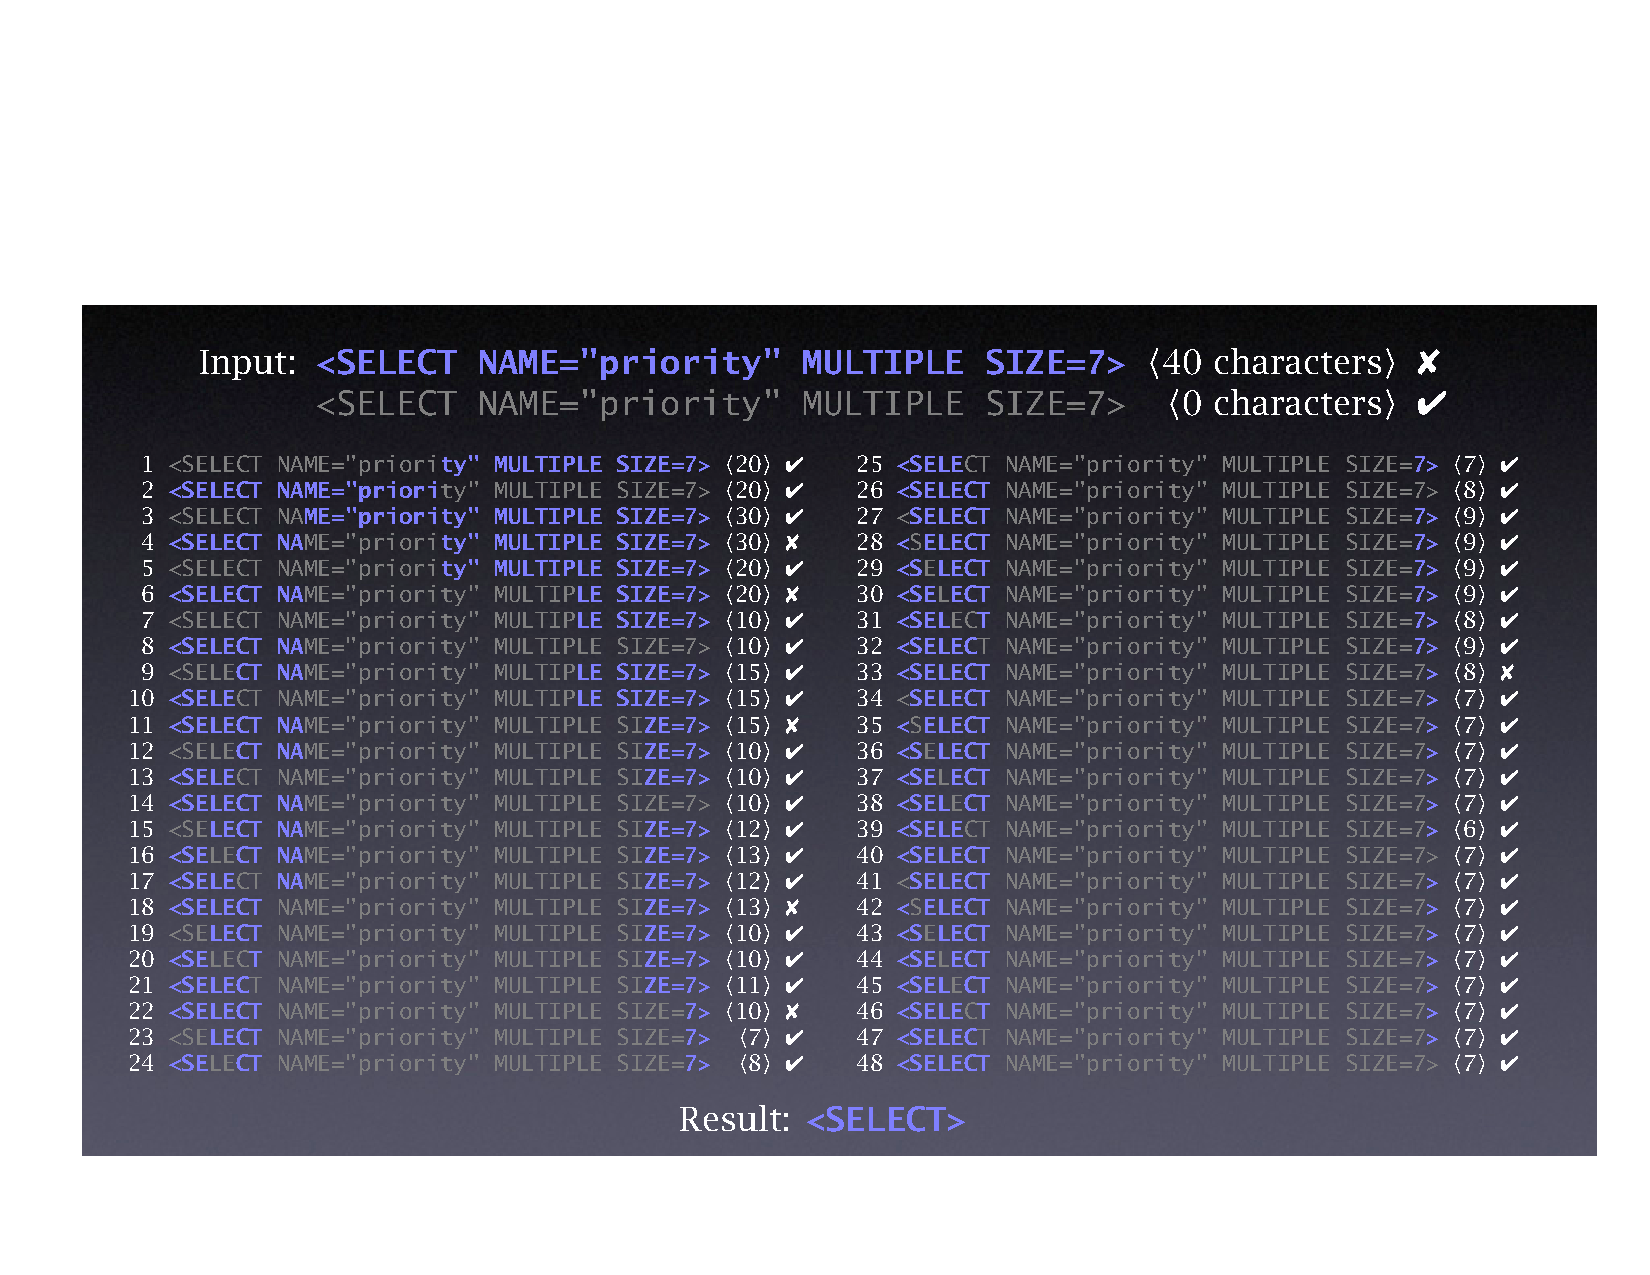
\includegraphics[width=1\textwidth]{images/DeltaDebuggingIlustration.pdf}
\end{minipage}
\caption{Delta Debugging: Algorithm and Illustration} 
\label{fig:deltadebugging} 
\end{figure*}


This idea of Delta Debugging was applied to isolate failure-inducing changes. It considers all line-level changes between the old and new program version as the candidate set without considering compilation dependences among those changes. In Zeller's seminal paper, {\textit``yesterday, my program worked, but today, it does not, why?''} Zeller demonstrates the application of DD to isolate program edits responsible for regression failures~\cite{Zeller1999}. DDD 3.1.2, released in December, 1998, exhibited a nasty behavioral change: When invoked with a the name of a non-existing file, DDD 3.1.2 dumped core, while its predecessor DDD 3.1.1 simply gave an error message. The DDD configuration management archive lists 116 logical changes between the 3.1.1 and 3.1.2 releases. These changes were split into 344 textual changes to the DDD source. After only 12 test runs and 58 minutes, the failure-inducing change was found: 
\begin{verbatim}
diff -r1.30 -r1.30.4.1 ddd/gdbinit.C 
295,296c296
<
< --- >
string classpath =
getenv("CLASSPATH") != 0 ? getenv("CLASSPATH") : ".";
string classpath = source view->class path();
\end{verbatim} 

When called with an argument that is not a file name, DDD 3.1.1 checks whether it is a Java class; so DDD consults its environment for the class lookup path. As an ``improvement'', DDD 3.1.2 uses a dedicated method for this purpose. Unfortunately, the source view pointer used is initialized only later, resulting in a core dump. 


\paragraph{Spectra-based fault localization.} Spectrum-based fault localization techniques such as Tarantula~\cite{Jones2002:tarantula} statistically compute suspiciousness scores for statements based on execution traces of both passed and failed test cases, and rank potential faulty statements based on the derived suspiciousness scores. Researchers have also introduced more suspiciousness computation measures to the realm of fault localization for localizing faulty statements~\cite{naish2011model, lo2010comprehensive} and also developed various automated tool-sets which embodies different spectrum-based fault localization techniques~\cite{tarantula-url, janssen2009zoltar}. However, such spectrum-based fault localization techniques are not scalable to large evolving software systems, as they compute spectra on all statements in each program version and do not leverage information about program edits between the old and new versions.

To address this problem, FaultTracer~\cite{zhang2011localizing} combines Chianti-style change impact analysis and Tarantula-style fault localization. To present a ranked list of potential failure-inducing edits, FaultTracer applies a set of spectrum-based ranking techniques to the affecting changes determined by Chianti-style change impact analysis. It uses a new enhanced call graph representation to measure test spectrum information directly for field-level edits and to improve upon the existing Chianti algorithm. The experimental results show that FaultTracer outperforms Chianti in selecting affected tests (slightly better) as well as in determining affecting changes (with an improvement of approximately 20\%). By ranking the affecting changes using spectrum-based profile, it places a real regression fault within a few atomic changes, significantly reducing developers’ effort in inspecting potential failure-inducing changes.

\subsection{Refactoring Validation} 
\label{sec:refactoringvalidation} 

Unlike other types of changes, refactoring validation is a special category of change validation. By definition, refactoring must guarantee behavior preservation and thus the old version's behavior could be compared against the new version's behavior for behavior preservation. Regression testing is the most used strategy for checking refactoring correctness. However, a recent study finds that test suites are often inadequate ~\cite{Rachatasumrit2012:refactortest} and developers may hesitate to initiate or perform refactoring tasks due to inadequate test coverage~\cite{Kim2012:FSR}. Soares et al.~\cite{Soares:icse10} design and implement SafeRefactor that uses randomly generated test suites for detecting refactoring anomalies. 

Formal verification is an alternative for avoiding refactoring anomalies~\cite{Mens2004:SSR}. Some propose rules for guaranteeing semantic preservation~cite{cornelio2010sound}, use graph rewriting for specifying refactorings~\cite{mens2005formalizing}, or present a collection of refactoring specifications, which guarantee the correctness by construction~\cite{overbey2010collection}. However, these approaches focus on improving the correctness of automated refactoring through formal specifications only. Assuming that developers may apply refactoring manually rather, Schaeffer et al.~validate refactoring edits by comparing data and control dependences between two program versions~\cite{Schaefer2010:refactoring}. 

RefDistiller is a static analysis approach~\cite{Alves2017:refdistiller,Alves:2014:RRA:2635868.2661674} to support the inspection of manual refactorings. It combines two techniques. First, it applies predefined templates to identify potential missed edits during manual refactoring. Second, it leverages an automated refactoring engine to identify extra edits that might be incorrect, helping to  determine the root cause of detected refactoring anomalies. GhostFactor~\cite{geManual2014} checks the correctness of manual refactoring, similar to RefDistiller. Another approach by Ge and Murphy-Hill~\cite{emersoncodereview:2014chase} helps reviewers by identifying applied refactorings and letting developers examine them in isolation by separating pure refactorings. 



